\section{Resultados}
A continuación se presentaran los resultados otenidos en la práctica de las distintas mediciones para cada tipo de carga, no lineal (capacitiva, inductiva) y lineal (resistiva).

\subsection{Ejecución del Ensayo con Carga Lineal}

Se energizó el circuito ajustando el VARIAC hasta obtener la tensión nominal y se varió la carga resistiva en distintos niveles (desde 1 kW hasta 200 W), registrando para cada uno los valores de tensión ($V$), corriente ($I$) y potencia activa ($P$) tanto en el lado de baja como de alta tensión. Las formas de onda de tensión y corriente fueron capturadas con el osciloscopio mediante resistencias shunt ($R_s$), evidenciando su comportamiento senoidal. Los resultados se muestran en la Tabla~\ref{tab:resultados_transformador}. En la Figura~\ref{fig:curva} se presenta la curva de voltaje vs corriente con carga lineal, mientras que en las Figuras~\ref{fig:onda_primario} y \ref{fig:onda_resistiva} se muestran las formas de onda en el primario y en la carga resistiva, respectivamente.

\begin{table}[H]
    \centering
    \caption{Mediciones con carga lineal}
    \label{tab:resultados_transformador}
    \begin{tabular}{ccccccc}
        \toprule
        \textbf{Carga [W]} & \multicolumn{3}{c}{\textbf{Baja Tensión}} & \multicolumn{3}{c}{\textbf{Alta Tensión}} \\
        \cmidrule(lr){2-4} \cmidrule(lr){5-7}
        & $V_1$ [V] & $I_1$ [A] & $P_1$ [W] & $V_2$ [V] & $I_2$ [A] & $P_2$ [W] \\
        \midrule
        1 kW  & $110 \pm 2$ & $13 \pm 0,5$ & $304 \pm 40$ & $220 \pm 5$ & $4 \pm 0,5$   & $864 \pm 1$ \\
        800 W & $110 \pm 2$ & $8 \pm 0,5$  & $152 \pm 40$ & $215 \pm 5$ & $4 \pm 0,5$   & $720 \pm 1$ \\
        600 W & $108 \pm 2$ & $6 \pm 0,5$  & $120 \pm 40$ & $215 \pm 5$ & $2 \pm 0,5$   & $552 \pm 1$ \\
        400 W & $108 \pm 2$ & $3 \pm 0,5$  & $80 \pm 40$  & $220 \pm 5$ & $1 \pm 0,5$   & $372 \pm 1$ \\
        200 W & $108 \pm 2$ & $1 \pm 0,5$  & $40 \pm 40$  & $220 \pm 5$ & $0,5 \pm 0,5$ & $192 \pm 1$ \\
        \bottomrule
    \end{tabular}
\end{table}

\begin{center}
        \begin{figure}[H]
        \centering
        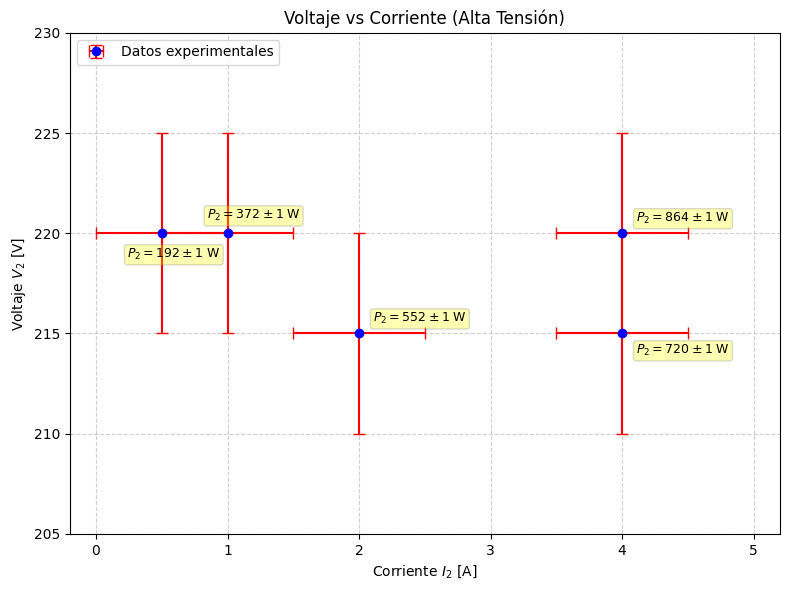
\includegraphics[width=0.65\textwidth]{imagenes/curva-voltaje-vs-corriente.png}
        \caption{Curva de Voltaje vs Corriente con carga lineal}
        \label{fig:curva}
        \end{figure}
    \end{center}

\begin{center}
        \begin{figure}[H]
        \centering
        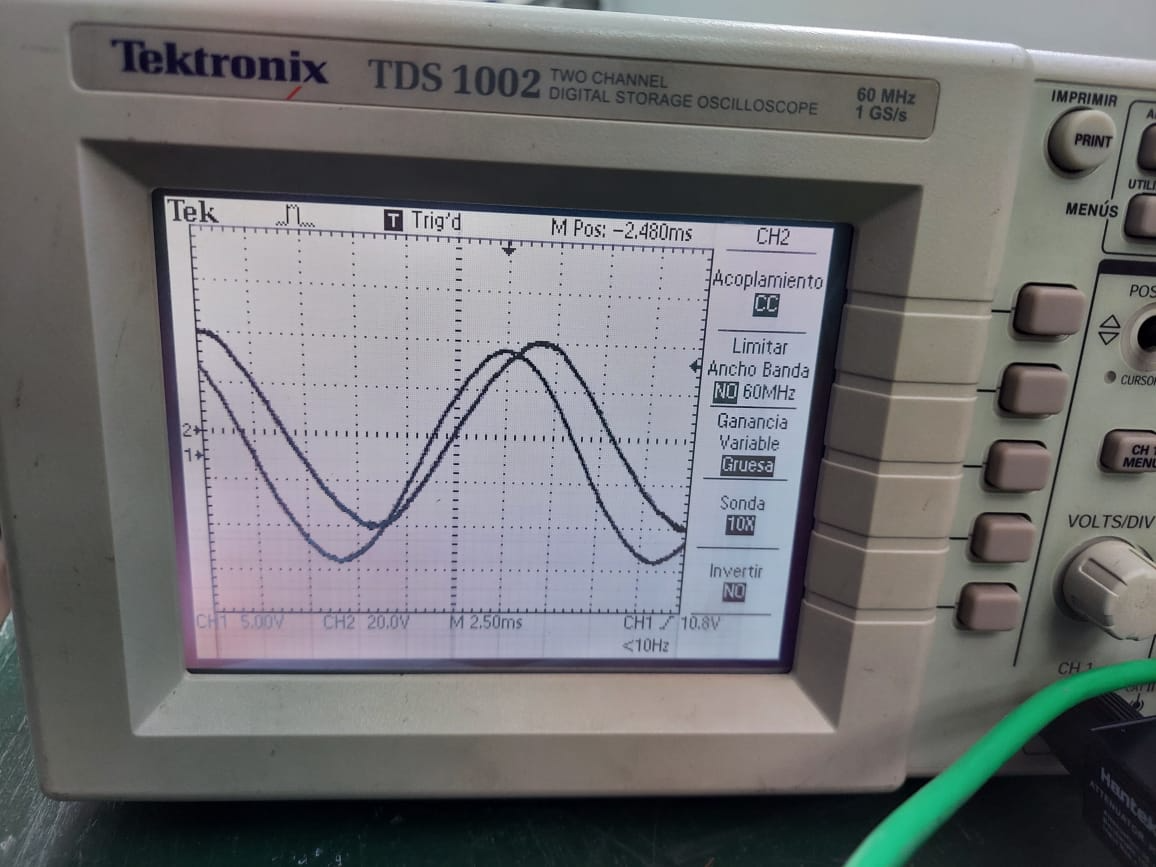
\includegraphics[width=0.8\textwidth]{imagenes/forma-de-onda-primario.png}
        \caption{Forma de onda en el primario con carga lineal}
        \label{fig:onda_primario}
        \end{figure}
    \end{center}

\begin{center}
        \begin{figure}[H]
        \centering
        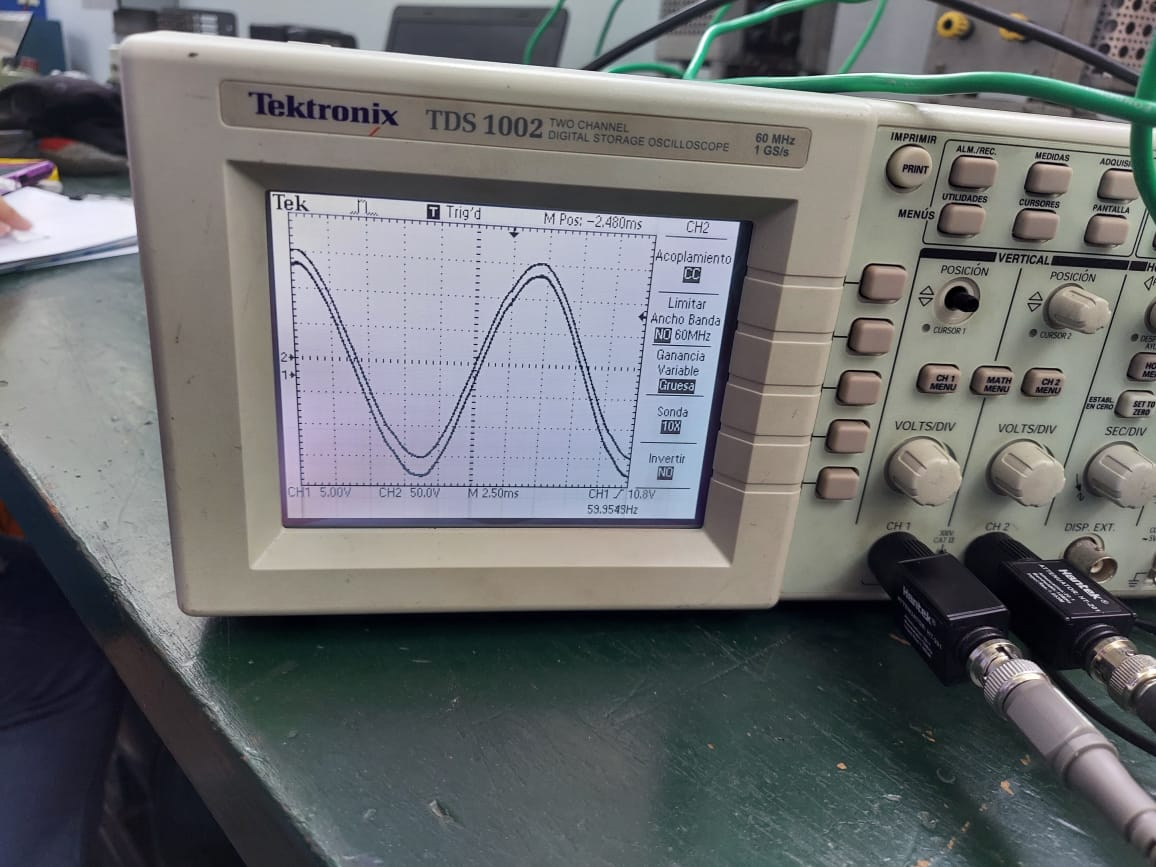
\includegraphics[width=0.8\textwidth]{imagenes/forma-de-onda-resistencia.png}
        \caption{Forma de onda en la carga resistiva}
        \label{fig:onda_resistiva}
        \end{figure}
    \end{center}

\subsection{Ejecución del Ensayo con Carga Capacitiva}

Para este ensayo se conectó el puente rectificador en el lado secundario del transformador para alimentar la carga no lineal conformada por un arreglo capacitivo-resistivo. Se tomaron las mediciones de los parámetros eléctricos con el osciloscopio y se observaron las variaciones en el factor de potencia y el contenido armónico inducido por la distorsión de la señal. La Tabla~\ref{tab:carga_capacitiva} y la Figura~\ref{fig:capacitiva} (forma de onda de corriente vs voltaje en la carga capacitiva) presentan los resultados obtenidos.

\begin{table}[H]
    \centering
    \caption{Medición con carga capacitiva}
    \label{tab:carga_capacitiva}
    \begin{tabular}{cccccc}
        \toprule
        \multicolumn{3}{c}{\textbf{Baja Tensión}} & \multicolumn{3}{c}{\textbf{Alta Tensión}} \\
        \cmidrule(lr){1-3} \cmidrule(lr){4-6}
        $V_1$ [V] & $I_1$ [A] & $P_1$ [W] & $V_2$ [V] & $I_2$ [A] & $P_2$ [W] \\
        \midrule
        $68,5 \pm 0,01$ & $8,0 \pm 0,5$ & $550 \pm 1$ & $126,4 \pm 0,01$ & $4,24 \pm 0,01$ & $450 \pm 1$ \\
        \bottomrule
    \end{tabular}
\end{table}

Con el propósito de evaluar el comportamiento del transformador ante una carga capacitiva, se determina la potencia aparente ($S_{\text{alta}}$) en el devanado de alta tensión. Esta magnitud representa la potencia total que fluye a través del equipo y se calcula mediante el producto de la tensión y la corriente medidas:

\begin{align}
    S_{\text{alta}} = V_{\text{alta}} \cdot I_{\text{alta}} \label{eq:s_alta}
\end{align}

\begin{align}
    \Delta S_{\text{alta}} = S_{\text{alta}} \cdot \left( \frac{\Delta V_{\text{alta}}}{V_{\text{alta}}} + \frac{\Delta I_{\text{alta}}}{I_{\text{alta}}} \right) \label{eq:delta_s_alta}
\end{align}

Seguidamente, se calcula el factor de potencia ($FP$), un indicador adimensional que expresa la relación entre la potencia activa ($P_{\text{alta}}$) que genera trabajo útil y la potencia aparente obtenida en el paso anterior:

\begin{align}
    FP = \frac{P_{\text{alta}}}{S_{\text{alta}}} \label{eq:fp}
\end{align}

\begin{align}
    \Delta FP = FP \cdot \left( \frac{\Delta P_{\text{alta}}}{P_{\text{alta}}} + \frac{\Delta S_{\text{alta}}}{S_{\text{alta}}} \right) \label{eq:delta_fp}
\end{align}

\begin{table}[H]
\centering
\caption{Resultados calculados para la potencia aparente y el factor de potencia en el lado de alta tensión con sus respectivas incertidumbres (Carga Capacitiva).}
\label{tab:resultados_alta_tension}
\vspace{0.2cm}
\begin{tabular}{l c c c}
\toprule
\textbf{Magnitud} & \textbf{Valor Calculado} & \textbf{Incertidumbre} & \textbf{Resultado Final} \\
\midrule
Potencia Aparente ($S_{\text{alta}}$) & $535,94 \text{ VA}$ & $\pm 1,3 \text{ VA}$ & $\mathbf{535,9 \pm 1,3 \text{ VA}}$ \\
Factor de Potencia ($FP$)             & $0,8397$              & $\pm 0,0039$         & $\mathbf{0,840 \pm 0,004}$ \\
\bottomrule
\end{tabular}
\end{table}

\begin{center}
        \begin{figure}[H]
        \centering  
        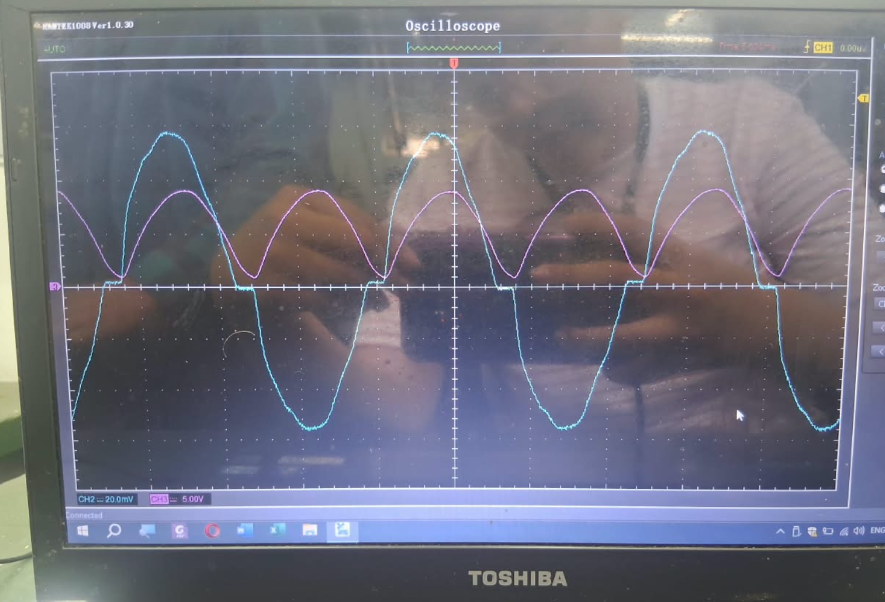
\includegraphics[scale=0.9]{imagenes/capacitiva.png}
        \caption{Forma de onda de Corriente vs Voltaje en una carga capacitiva 1000W lado de baja
tensión}
        \label{fig:capacitiva}
        \end{figure}
    \end{center}

\subsection{Ejecución del Ensayo con Carga Inductiva }

Al igual que en el caso capacitivo, se mantuvo el puente rectificador en el secundario, pero esta vez alimentando la carga inductiva. Se repitieron las mediciones de tensión, corriente y potencia, registrando la distorsión de la corriente debida a los armónicos generados por el rectificador. Los valores obtenidos se resumen en la Tabla~\ref{tab:carga_inductiva} y la forma de onda de corriente vs voltaje en la carga inductiva se muestra en la Figura~\ref{fig:inductiva}.

\begin{table}[H]
    \centering
    \caption{Mediciones con carga inductiva}
    \label{tab:carga_inductiva}
    \begin{tabular}{cccccc}
        \toprule
        \multicolumn{3}{c}{\textbf{Baja Tensión}} & \multicolumn{3}{c}{\textbf{Alta Tensión}} \\
        \cmidrule(lr){1-3} \cmidrule(lr){4-6}
        $V_1$ [V] & $I_1$ [A] & $P_1$ [W] & $V_2$ [V] & $I_2$ [A] & $P_2$ [W] \\
        \midrule
        $92 \pm 2$ & $7 \pm 0,5$ & $132 \pm 0,5$ & $180 \pm 10$ & $3 \pm 0,5$ & $624 \pm 1$ \\
        \bottomrule
    \end{tabular}
\end{table}

A fin de calcular la potencia aparente y el factor de potencia con sus respectivas incertidumbres, se procede de igual forma que en el análisis con carga capacitiva, utilizando las relaciones definidas en las ecuaciones \eqref{eq:s_alta}, \eqref{eq:delta_s_alta}, \eqref{eq:fp} y \eqref{eq:delta_fp}:

\begin{table}[H]
\centering
\caption{Resultados calculados para la potencia aparente y el factor de potencia en el lado de alta tensión (Carga Inductiva).}
\label{tab:resultados_inductiva}
\vspace{0.2cm}
\begin{tabular}{l c c c}
\toprule
\textbf{Magnitud} & \textbf{Valor Calculado} & \textbf{Incertidumbre} & \textbf{Resultado Final} \\
\midrule
Potencia Aparente ($S_{\text{alta}}$) & $540 \text{ VA}$ & $\pm 120 \text{ VA}$ & $\mathbf{540 \pm 120 \text{ VA}}$ \\
Factor de Potencia ($FP$)             & $1,155$            & $\pm 0,259$          & $\mathbf{1,16 \pm 0,26}$ \\
\bottomrule
\end{tabular}
\end{table}

\begin{center}
        \begin{figure}[H]
        \centering  
        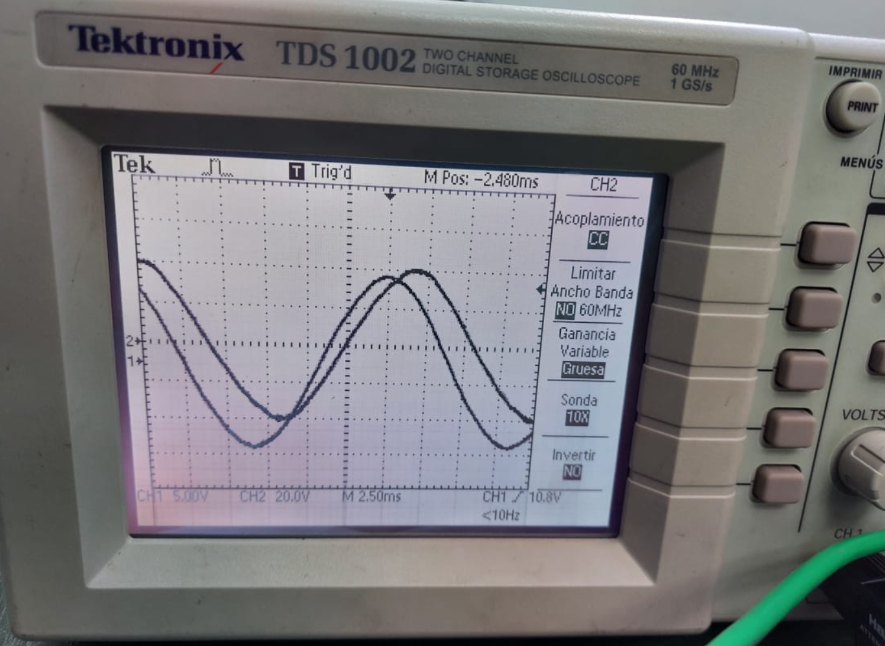
\includegraphics[scale=0.9]{imagenes/inductiva.png}
        \caption{Forma de onda de Corriente vs Voltaje en una carga inductiva 1000W lado de baja
tensión}
        \label{fig:inductiva}
        \end{figure}
    \end{center}